%---------- Quinto Capitulo ----------
\chapter{Desenvolvimento}\label{cha:desenvolvimento}
Este trabalho de conclusão de curso necessitou que fossem implementados uma aplicação servidora, o \textit{Broker}, que gerencia a escolha das aplicações que melhor atendem as configurações definidas pelo usuário; a aplicação para dispositivo móvel, onde o usuário realiza as configurações que deseja para cada tipo de serviço e que também consome esses serviços; e também alguns simuladores de provedores de serviço. Para armazenamento de dados, foi utilizado um banco de dados na nuvem. A Figura \ref{fig:arquitetura} mostra a organização da arquitetura do projeto, onde podemos ver um dispositivo móvel conectado à Internet, alguns provedores de serviços, o \textit{Broker} e o banco de dados utilizado pelo \textit{Broker}.
Nessa arquitetura o cliente realiza a requisição do uso do serviço através do \textit{Broker}, que é o encarregado de escolher qual é o serviço que atende aos requisitos do usuário, como no exemplo apresentado pela Figura \ref{fig:arquiteturaexplicada} que explica o funcionamento da arquitetura.

\begin{figure}[!htb]
  \centering
  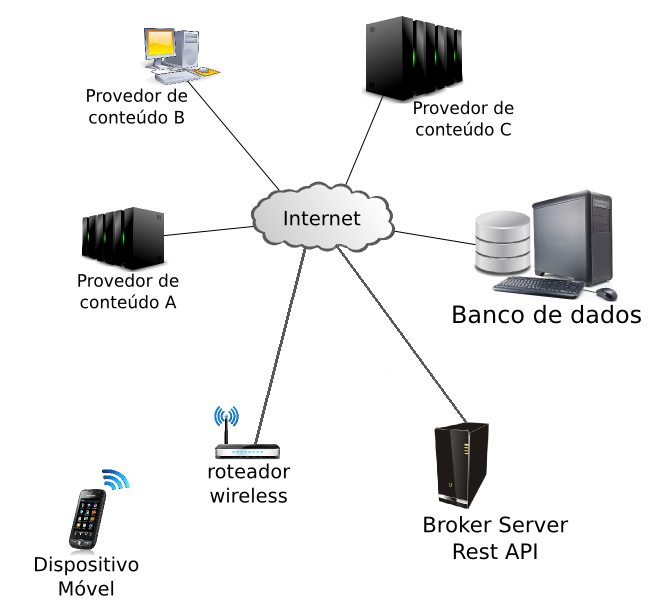
\includegraphics[width=.7\textwidth]{arquitetura.png} % <- formatos PNG, JPG e PDF
  \caption[Arquitetura do projeto]{Arquitetura do projeto}
  \label{fig:arquitetura}
\end{figure}

\begin{figure}[!htb]
  \centering
  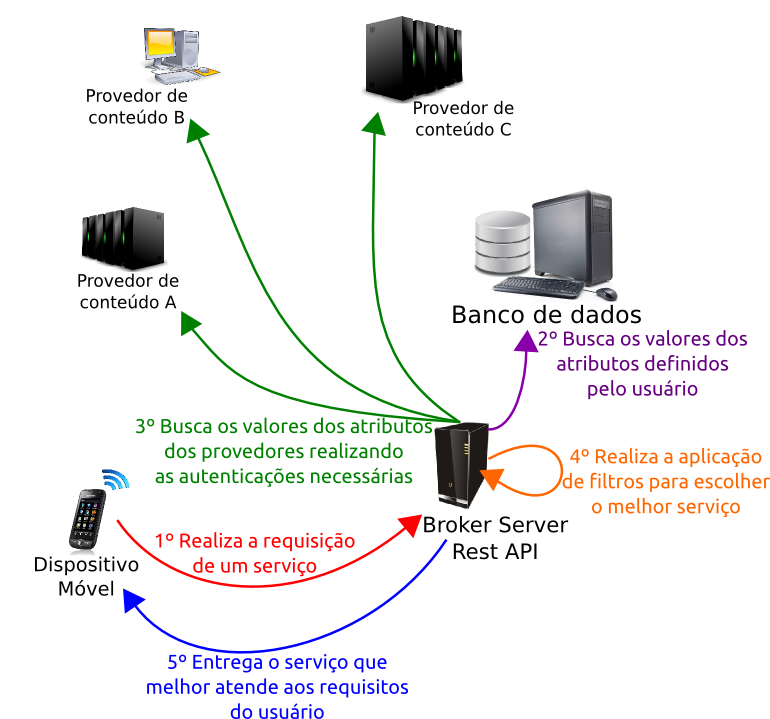
\includegraphics[width=.7\textwidth]{arquiteturaexplicada.png} % <- formatos PNG, JPG e PDF
  \caption[Explicação do funcionamento da arquitetura do projeto]{Explicação do funcionamento da arquitetura do projeto}
  \label{fig:arquiteturaexplicada}
\end{figure}

%----------------- Serviços -----------------
\section{Serviços}
Os dispositivos móveis são utilizados diariamente como 'computadores de bordo' pelas pessoas, são meios de obter informações sobre o que está acontecendo. No decorrer do dia a pessoa utiliza seu dispositivo para consultar email, trocar mensagens, consultar as condições do trânsito, condições climáticas, ler notícias do jornal, obter rotas, ouvir música e muito mais.

Muitos desses serviços necessitam que o usuário tenha uma conta registrada e que seja autenticado antes de utilizá-lo. E também são genéricos o suficiente para oferecer o serviço ao maior número de usuários possíveis.

Devido a essa característica de oferecer um serviço genérico, o usuário deve aplicar filtros na aplicação do serviço para obter a informação necessária.

Vamos utilizar como exemplo uma consulta ao serviço de metereologia, então o usuário:
\begin{enumerate}
  \item Abre o navegador de internet;
  \item Abre um site de busca;
  \item Procura pela palavra metereologia;
  \item Escolhe um dos serviços na lista;
  \item Tenta usar o serviço, se não conseguir volta ao passo anterior;
  \item Se necessário, cria uma conta e autentica-se no serviço;
  \item Aplica os filtros necessários;
  \item Obtém as informações.
\end{enumerate}

Dependendo do tipo de serviço, esses passos serão sempre repetidos, principalmente o passo de autenticação, e as informações do usuário vão estar sempre expostas numa rede sem fio onde qualquer pessoa mal intensionada, com ferramentas adequadas, poderá capturá-las. E é esse tipo de problema que queremos resolver.

\subsection{Implementação de um serviço como prova de conceito}
Como as implementações dos serviços não fazem parte do escopo deste trabalho, foram implementados apenas serviços incompletos que simulam o funcionamento de um serviço real. No caso, foram implementados três serviços que oferecem dados metereológicos falsos, sendo que em um deles é necessário que o usuário tenha sido previamente cadastrado, assim para obter as informações do serviço, precisará realizar a autenticação.

Esses serviços foram implementados como \textit{Web Services} \sigla{REST}{Representational State Transfer} (\textit{Representational State Transfer}), assim precisamos apenas realizar uma chamada à interface adequada para obter a resposta.

Existem provedores de serviços reais que oferecem esse tipo de API, como por exemplo o \textit{OpenWeatherMap}\footnote{openweathermap.org/api}, não é gratuito e é um serviço rico em informações. Para utilizar o serviço pode ser realizado um cadastro simples que possui um uso limitado, nesse cadastro o usuário recebe uma chave que pode ser usado numa requisição como no exemplo a seguir:

\url{http://api.openweathermap.org/data/2.5/weather?q=Maringa,br&APPID=CHAVE_DO_USUARIO}

Essa consulta retornaria um JSON com muitas informações da cidade de Maringá, como as coordenadas de localização da cidade e os dados metereológicos de temperatura, humidade, pressão, etc. Logo abaixo pode ser visto um resumo dessas informações:

\begin{verbatim}
    { "coord":{
        "lon": -51.94
        "lat": -23.43
      }, "weather": {
        "description": "light rain",
        "temp": 30,
        "pressure": 1011,
        "humidity": 74,
        "temp_min": 30,
        "temp_max": 30,
        "wind": {
          "speed": 2.1
        }, "sys": {
          "name": "Maringa",
          "country": "BR"
        }
      }
    }
\end{verbatim}

Os serviços que foram implementados para este trabalho seguem uma linha semelhante, eles respondem a requisições POST nos endereços:
\begin{enumerate}
  \item \url{http://weather-provider.herokuapp.com/weather}
  \item \url{http://weather-nd-provider.herokuapp.com/weather}
  \item \url{http://weather-rd-provider.herokuapp.com/weather}
\end{enumerate}

Sendo que o primeiro necessita que o usuário seja registrado no serviço e que realize a autenticação para poder utilizá-lo. Para realizar o registro no serviço é necessário uma chamada simples à interface de registro:

\url{http://weather-provider.herokuapp.com/register/EMAIL_DO_USUARIO/UMA_SENHA}

Como já foi dito, a implementação dos serviços não fazem parte do escopo do trabalho, então foram criadas apenas as interfaces REST necessárias para o funcionamento. Assim, as chamadas às interfaces destes serviços respondem com uma lista com objetos JSON com dados fictícios sobre o clima de algumas cidades do Paraná. Como no exemplo logo abaixo, onde temos dados metereológicos das cidades de Curitiba e Maringá, nesses objetos temos dados como temperatura, humidade e como está o céu:

\begin{verbatim}
  [{  "provider": "First Weather Provider",
      "city": "Curitiba",
      "temperature": 15,
      "Humidity": 47,
      "sky": "weather-cloudy",
      "update": "2016-01-28T03:06:06.756Z"
  },{ "provider": "First Weather Provider",
      "city": "Maringá",
      "temperature": 7,
      "Humidity": 33,
      "sky": "weather-rainy",
      "update": "2016-01-28T18:12:10.002Z"
  }...]
\end{verbatim}

Ao obter esses dados, o \textit{Broker} trabalhará sobre eles e escolherá as informações do serviço que melhor atendem às preferências do usuário.

\subsection{Serviços disponíveis}
O \textit{Broker} entrega à aplicação do dispositivo móvel uma lista com alguns tipos de serviços e seus atributos de preferências, que são:

\begin{itemize}
  \item Games
    \begin{itemize}
      \item Amount of users
    \end{itemize}
  \item Video
    \begin{itemize}
      \item Amount of videos
    \end{itemize}
  \item News
    \begin{itemize}
      \item City
      \item Last update
      \item Closer to me
    \end{itemize}
  \item Music
    \begin{itemize}
      \item Amount of music
    \end{itemize}
  \item Weather
    \begin{itemize}
      \item City
      \item Last update
    \end{itemize}
\end{itemize}

%----------------- Aplicação -----------------
\section{A aplicação para dispositivos móveis}
A implementação do aplicativo para dispositivo móvel utilizou o Ionic \textit{Framework}. Dessa forma, a aplicação foi desenvolvida com o uso das Linguagens Javascript, HTML e CSS.

O Ionic \textit{Framework} foi desenvolvido sobre outro \textit{framework}, o Apache Cordova, o que idealmente permite que a aplicação desenvolvida possa ser executada em todas as plataformas de dispositivo móvel à qual o Apache Cordova oferece suporte.

Abaixo é apresentada a Figura \ref{fig:ionicarch} que mostra a organização da arquitetura do \textit{framework}. Essa figura é meramente ilustrativa, pois nas últimas camadas temos um número bem maior de funcionalidades nos dispositivos, assim como um número maior de sistemas operacionais alvos do Apache Cordova.

\begin{figure}[!htb]
  \centering
  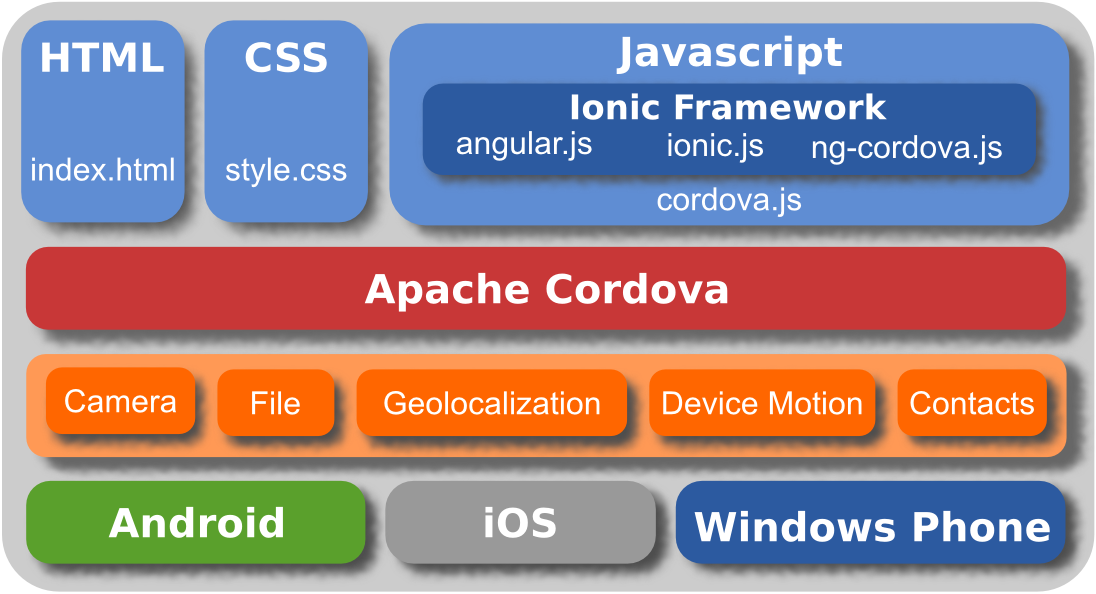
\includegraphics[width=.8\textwidth]{ionicarch.png} % <- formatos PNG, JPG e PDF
  \caption[Arquitetura do Ionic Framework]{Arquitetura do Ionic Framework}
  \label{fig:ionicarch}
\end{figure}

A implementação e os testes da aplicação tiveram como SO alvo apenas o Android.

A aplicação foi desenvolvida com uma interface intuitiva, com ícones expressivos para que o usuário tivesse uma experiência agradável e sem transtornos.

As configurações necessárias são mínimas e qualquer pessoa envolvida no contexto da aplicação conseguiria realizá-las em poucos passos e já teria a aplicação em funcionamento em seu aparelho.

O Apêndice A apresenta um modelo de navegação na aplicação.

\subsection{Configurando um serviço}
Como o objetivo da aplicação no dispositivo móvel é apresentar ao usuário o melhor serviço que respeite as suas preferências, é necessário que esses atributos sejam cadastrados de alguma forma. Nos passos a seguir será mostrado como configurar um desses serviços, no caso, será utilizado o serviço de metereologia (\textit{Weather}).

Depois de realizar as configurações iniciais, como:
\begin{enumerate}
  \item cadastrar o endereço do \textit{Broker};
  \item cadastrar o usuário;
  \item realizar \textit{login} na aplicação
\end{enumerate}

o usuário navegará até a aba de serviços, exibido na Figura \ref{fig:navegar}

\begin{figure}[!htb]
  \centering
  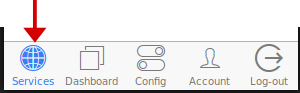
\includegraphics[width=.4\textwidth]{navegar.png} % <- formatos PNG, JPG e PDF
  \caption[Aba de serviços]{Aba de serviços}
  \label{fig:navegar}
\end{figure}

o usuário deverá tocar no botão de configuração do endereço do provedor de serviço, em destaque na Figura \ref{fig:configurl}

\begin{figure}[!htb]
  \centering
  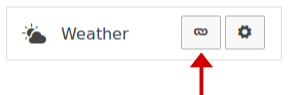
\includegraphics[width=.5\textwidth]{configurl.png} % <- formatos PNG, JPG e PDF
  \caption[Botão para configuração dos endereços dos serviços]{Botão para configuração dos endereços dos serviços}
  \label{fig:configurl}
\end{figure}

e realizar a configuração do endereço, preenchendo os campos como os exibidos na Figura \ref{fig:registerurl}, se necessário, adicionar os dados de autenticação do provedor de serviço, essas serão as informações que o servidor utilizará para que sejam realizadas as autenticações necessárias de forma transparente.

\begin{figure}[!htb]
  \centering
  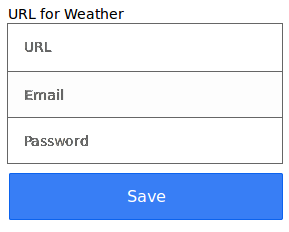
\includegraphics[width=.4\textwidth]{registerurl.png} % <- formatos PNG, JPG e PDF
  \caption[Cadastro do endereço do provedor de serviço e dados de autenticação]{Cadastro do endereço do provedor de serviço e dados de autenticação}
  \label{fig:registerurl}
\end{figure}

Logo em seguida, o usuário deverá configurar suas preferências, tocando no botão em destaque na Figura \ref{fig:configprefs}

\begin{figure}[!htb]
  \centering
  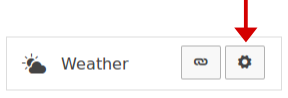
\includegraphics[width=.5\textwidth]{configprefs.png} % <- formatos PNG, JPG e PDF
  \caption[Botão para configuração das preferências do usuário]{Botão para configuração das preferências do usuário}
  \label{fig:configprefs}
\end{figure}

e realizar a configuração das preferências, que no caso para o tipo de serviço \textit{Weather} o usuário marcará se precisa que as informações sejam as mais atualizadas possíveis e qual a sua cidade de preferência, como mostrado na Figura \ref{fig:weatherprefs}

\begin{figure}[!htb]
  \centering
  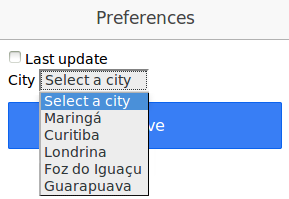
\includegraphics[width=.4\textwidth]{weatherprefs.png} % <- formatos PNG, JPG e PDF
  \caption[Configuração das preferências do usuário]{Configuração das preferências do usuário}
  \label{fig:weatherprefs}
\end{figure}

Cadastrando esses dados, o usuário não precisará mais informar o endereço do provedor de serviço nem seus dados de autenticação, ele será autenticado de forma transparente e receberá na aba \textit{Dashboard}, em destaque na Figura \ref{fig:dashboard}, as informações do provedor que melhor atender as suas preferências.

\begin{figure}[!htb]
  \centering
  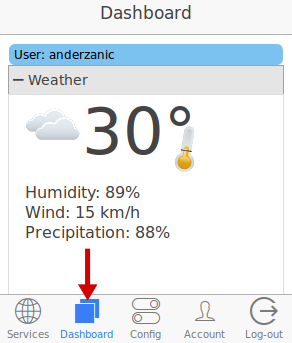
\includegraphics[width=.4\textwidth]{dashboard.png} % <- formatos PNG, JPG e PDF
  \caption[Aba \textit{Dashboad} que exibe os serviços configurados]{Aba \textit{Dashboad} que exibe os serviços configurados}
  \label{fig:dashboard}
\end{figure}

Nessa aba são exibidos apenas os serviços que tiveram as preferências configuradas.

\subsection{Angular.js}
Angular.js foi desenvolvido pela Google. É um \textit{framework} para desenvolvimento de aplicações web \textit{Single Page Applications}, onde todas as páginas da aplicação são desenvolvidas como \textit{templates} e são injetadas na página principal quando requisitadas, a Figura \ref{fig:ngview} exibe um exemplo de como isso funciona, no exemplo da figura a \textit{tag} HTML <ng-view> é o espaço onde as \textit{templates} serão renderizadas.

\begin{figure}[!htb]
  \centering
  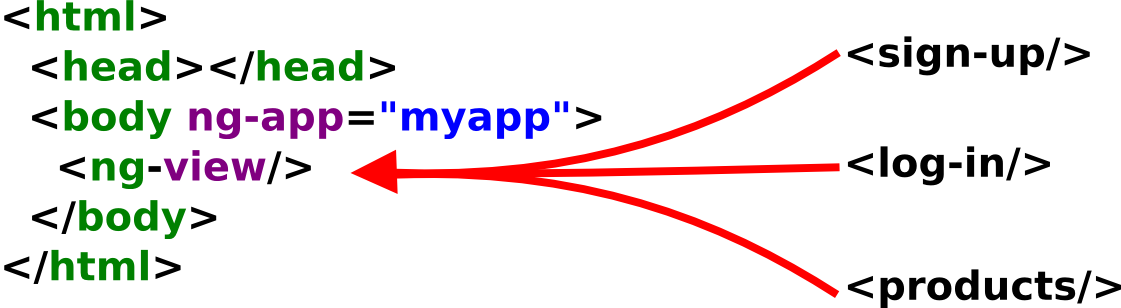
\includegraphics[width=.7\textwidth]{ngview.png} % <- formatos PNG, JPG e PDF
  \caption[Exemplo do funcionamento de uma \textit{Single Page Applications}]{Exemplo do funcionamento de uma \textit{Single Page Applications}}
  \label{fig:ngview}
\end{figure}

Uma característica muito importante do Angular.js é que ele estende o vocabulário padrão do HTML, permitindo que sejam desenvolvidos sistemas com um código muito mais expressivo no \textit{front-end}.

Como por exemplo o uso de uma \textit{tag} HTML como: 
\begin{verbatim}
                  <genero />
\end{verbatim}

é mais expressivo do que:

\begin{verbatim}
                  <label>Gênero: </label>
                  <select name="genero">
                    <option value="M">Masculino</option>
                    <option value="F">Feminino</option>
                  </select>
\end{verbatim}

Além desse ganho na expressividade, a modularização e reúso de código acontece efetivamente, o que diminui o tempo de desenvolvimento e aumenta a qualidade das aplicações.

Outro recurso muito interessante é o \textit{Two-Way Data Binding}, que permite a sincronização automática dos dados da \textit{view} com o modelo sem a manipulação direta do DOM pelo desenvolvedor.

\begin{figure}[!htb]
  \centering
  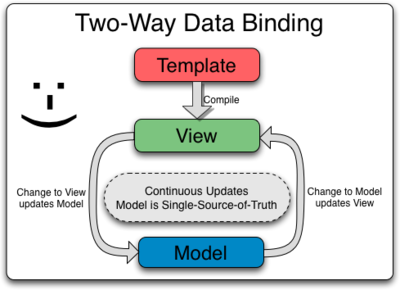
\includegraphics[width=.5\textwidth]{databinding.png} % <- formatos PNG, JPG e PDF
  \caption[Sincronização automática do \textit{model} e da \textit{view}]{Sincronização automática do \textit{model} e da \textit{view}. Fonte: \cite{angulardb}}
  \label{fig:twoway}
\end{figure}

\subsection{Construção dinâmica de formulário}
Um dos desafios enfrentados durante a implementação da aplicação para o dispositivo móvel foi a construção do formulário que exibe as configurações das preferências do usuário para cada serviço. Como cada serviço apresenta um determinado conjunto de atributos, iria ser necessário a implementação de uma \textit{template} para cada tipo de serviço, isso iria aumentar a complexidade de atualizações e manutenções de código.

Para evitar esses problemas e outros que poderiam surgir, como por exemplo: uma mudança nos atributos do serviço, foi desenvolvido um componente, que constrói o formulário de configuração de preferências de acordo com parâmetros enviados pelo \textit{Broker}.

Por exemplo, podemos enviar esses objetos JSON com essas configurações abaixo ao dispositivo móvel e ele produzirá um formulário como a Figura \ref{fig:geracaoauto}.
\begin{verbatim}
          { "element": "input",
            "type": "text",
            "name": "email",
            "label": "Email"
          },
          { "element": "input",
            "type": "password",
            "name": "password",
            "label": "Password" }
\end{verbatim}

\begin{figure}[!htb]
  \centering
  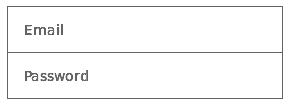
\includegraphics[width=.4\textwidth]{geracaoauto.png} % <- formatos PNG, JPG e PDF
  \caption[Geração automática de formulário]{Geração automática de formulário}
  \label{fig:geracaoauto}
\end{figure}

%----------------- Broker -----------------
\section{O \normalfont\itshape Broker}
O \textit{Broker} foi implementado como um \textit{Web Services} REST que expõe as interfaces necessárias para a aplicação cliente instalada no dispositivo móvel. A arquitetura REST foi a escolhida devido a sua simplicidade e segundo \cite{fielding2000architectural} a arquitetura REST é simples pois é uma abstração dos elementos de uma arquitetura web.
\begin{citacao}
O estilo REST é uma abstração dos elementos arquitectônicos dentro de um sistema hipermídia distribuído. REST ignora os detalhes da implementação do componente e da sintaxe do protocolo, a fim de se concentrar nos papéis dos componentes, as restrições sobre a sua interação com outros componentes, e sua interpretação de dados significativos. Ela abrange as restrições fundamentais sobre os componentes, conectores e dados que definem a base da arquitetura Web e, portanto, a essência do seu comportamento como um aplicativo baseado na rede. \cite{fielding2000architectural}
\end{citacao}
Em outras palavras, REST é um alternativa leve para \textit{Web Services} pois ele expõe apenas interfaces com os métodos padrão do \sigla{HTTP}{Hypertext Transfer Protocol} (\textit{Hypertext Transfer Protocol}), que também são conhecidos como verbos: GET e POST. Além desses dois existem os PUT, DELETE, HEAD e OPTIONS\footnote{O significado de cada um desses métodos é definido na especificação do HTTP, juntamente com algumas garantias sobre o seus comportamentos}.

As interfaces que o servidor \textit{Broker} expõe aceitam e respondem objetos JSON, como por exemplo uma chamada GET ao método \textit{types} que responde uma lista com os tipos de serviços disponíveis e suas configurações.
Se fizermos essa requisição \url{http://brokerserver.herokuapp.com/types} à API REST, teremos como resultado uma lista de objetos JSON como no exemplo da Figura \ref{fig:jsonservicos}, onde temos no destaque em vermelho o tipo do serviço, e em azul os dados que serão necessários para a construção do formulário onde o usuário configura as prefêrencias para o serviço:

\begin{figure}[!htb]
  \centering
  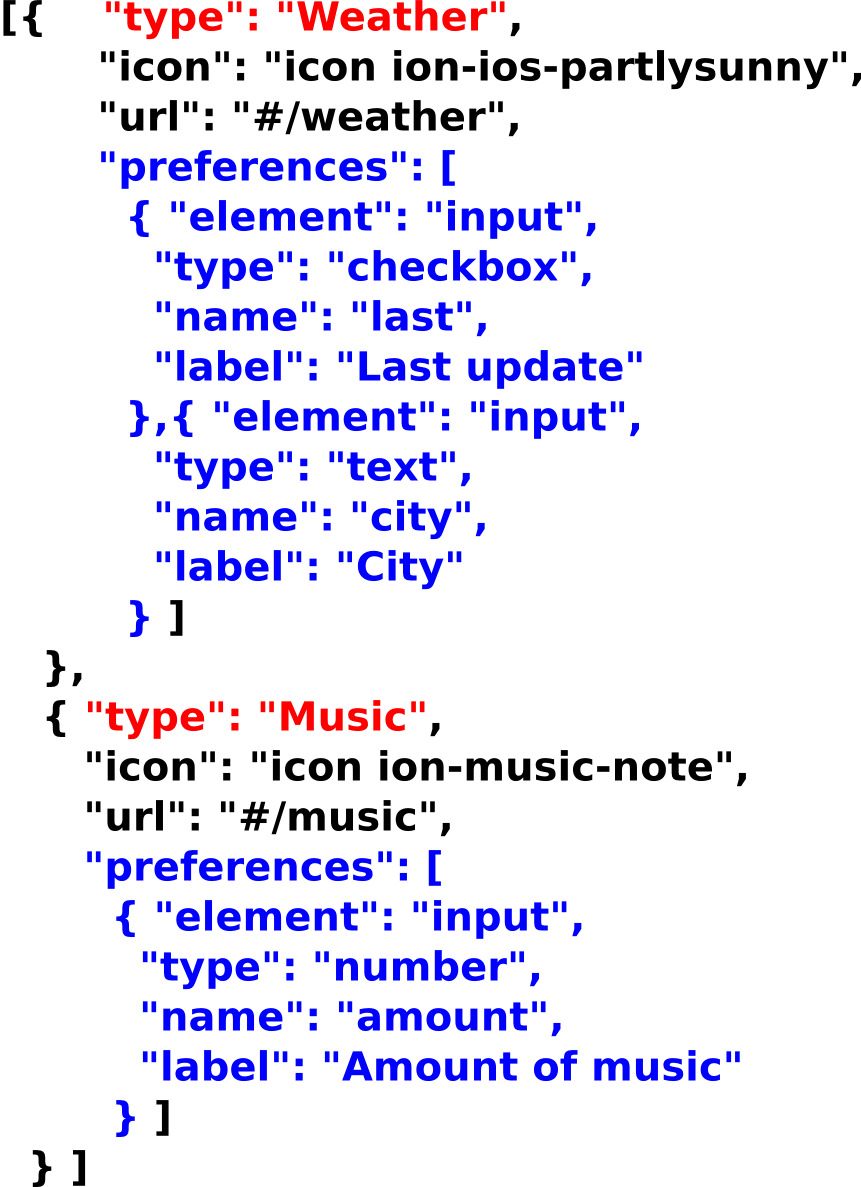
\includegraphics[width=.4\textwidth]{jsonservicos.png} % <- formatos PNG, JPG e PDF
  \caption[Objetos JSON retornados na requisição]{Objetos JSON retornados na requisição}
  \label{fig:jsonservicos}
\end{figure}

No evento de \textit{login} da aplicação do dispositivo móvel, é feita uma chamada POST ao método \textit{login} do \textit{Broker}, os parâmetros são enviados ao servidor no corpo da mensagem, como podemos notar na Figura \ref{fig:logindebug}, onde a aplicação foi executada em um navegador de internet com o console de \textit{debug} aberto.

\begin{figure}[h]
  \center
  \subfigure{
\includegraphics[width=.4\textwidth]{login.png}}
  \qquad
  \subfigure{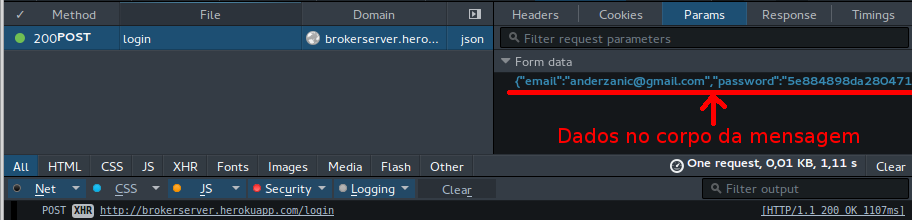
\includegraphics[width=1.1\textwidth]{debug.png}}
  \caption[\textit{Debug} da simulação de um \textit{login} na aplicação móvel]{\textit{Debug} da simulação de um \textit{login} na aplicação móvel}
  \label{fig:logindebug}
\end{figure}

Ao apertar o botão \textit{'Log in'} na aplicação móvel, a \sigla{URL}{Uniform Resource Locator} (\textit{Uniform Resource Locator}) \url{
http://brokerserver.herokuapp.com/login} foi chamada com os parâmetros \textit{email} e \textit{password} sendo enviados no corpo da mensagem.

\subsection{Autenticação transparente}

A Figura \ref{fig:registerurl} apresenta a tela onde o usuário cadastra o endereço dos provedores de serviço para cada tipo de serviço, além do endereço, são cadastrados também os dados de autenticação do usuário no provedor de serviço, esses dados são registrados no banco de dados que o \textit{Broker} utiliza e são recuperados para realizar a autenticação no provedor de serviço quando necessário.

Dessa forma o usuário não precisa informar dados de autenticação sempre que precisar utilizar o serviço, pois o \textit{Broker} irá realizar a autenticação no provedor de serviço de forma automática.

\subsection{Adicionando novos serviços}
O \textit{Broker} é o sistema encarregado de realizar a análise das preferências do usuário e deve cruzar essas informações com os estados dos provedores de serviço para poder decidir qual é o serviço que melhor atende aos requisitos do usuário.

Dependendo da linguagem de programação escolhida para resolver esse tipo de problema, pode ser que sejam necessárias muitas linhas de código para que seja alcançado um algoritmo adequado.

A característica funcional do Javascript foi um fator relevante pois foram utilizadas funções de alta ordem, funções que podem ser passadas como parâmetros para outras funções, e elas auxiliaram na resolução do problema com um código simples, limpo e elegante. Abaixo temos um exemplo do uso de funções de alta ordem em Javascript.

Suponha que temos uma lista de objetos e é preciso escolher um desses objetos, em Javascript podemos implementar uma função que funcionará como um predicado, e todos os objetos que responderem \textit{"verdade"} a esse predicado, serão escolhidos.

\begin{verbatim}
      var lista = [ {"cidade": "Maringá", "Estado":"PR"},
                    {"cidade": "Curitiba", "Estado":"PR"} ];
      var predicado = function(candidato){
                        return candidato.cidade === "Maringá";
                      };
      var resultado = lista.filter(predicado);
      console.log(resultado);
      // Imprime no console: [{"cidade": "Maringá", "Estado":"PR"}]
\end{verbatim}

Esse é um exemplo bem simples, mas a função de predicado pode ter a complexidade necessária e ainda assim o código que aplica o predicado se manterá sempre simples e além disso essa função poder ser modularizada transformado-se em um \textit{plugin} que poderá ser aplicado onde for necessário.

A Figura \ref{fig:novosservicos} apresenta um exemplo dessa situação, onde na Figura 'a)' o cliente realiza a consulta do serviço \textit{weather} e o \textit{Broker} utiliza o predicado \textit{weather} para filtrar os resultados obtidos, e na Figura 'b)' onde o predicado (\textit{news}) deve ser implementado.

\begin{figure}[h]
  \center
  \subfigure[fig:servicoweather][Predicado \textit{weather}]{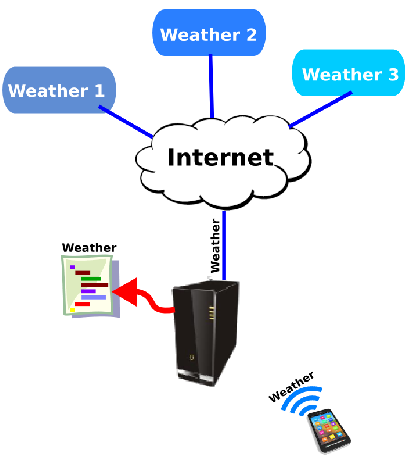
\includegraphics[width=.4\textwidth]{servicoweather.png}}
  \qquad
  \subfigure[fig:serviconews][Predicado \textit{news}]{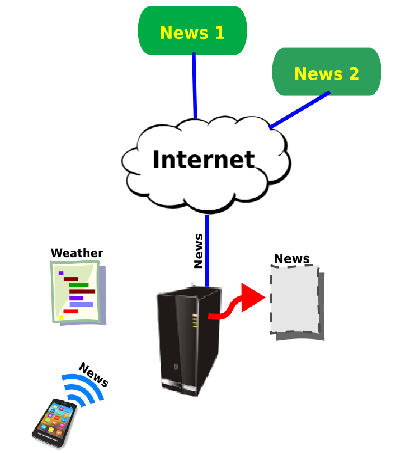
\includegraphics[width=.4\textwidth]{serviconews.png}}
  \caption[Funcionamento do uso dos predicados]{Funcionamento do uso dos predicados}
  \label{fig:novosservicos}
\end{figure}

No caso do \textit{Broker} isso foi fundamental pois cada vez que um novo serviço for ser oferecido será apenas necessário implementar o predicado, baseado nos atributos do serviço, e realizar o registro desse novo predicado no servidor, com a adição de uma única linha de código:

\begin{verbatim}
      var novoservico = require('./novoservico.js');
\end{verbatim}

\subsection{Jasmine \normalfont\itshape Framework}
Jasmine é um \textit{framework} para testes de códigos Javascript. Como Javascript é uma linguagem de tipagem dinâmica, é necessário que sejam implementados testes que possam aumentar a confiança de que as funções estão respondendo de maneira correta.
Dessa forma, algumas funções do \textit{Broker} tiveram testes implementados.

O \textit{framework} Jasmine suporta a técnica ágil "Desenvolvimento Guiado por Comportamento", conhecido pela sigla em inglês BDD, é uma técnica que encoraja o envolvimento entre os desenvolvedores, setores de qualidade e pessoas sem conhecimento técnico e que dominam a regra do negócio. Os testes são criados utilizando a linguagem nativa e a codificação do teste em Javascript, o uso da linguagem nativa auxilia o desenvolvedor a manter o foco na razão pela qual o código deve ser implementado.
Logo abaixo temos um exemplo de um teste com Jasmine.

Antes da execução de cada teste, que está implementado dentro de cada declaração "it('mensagem', function(){});", é executado o código declarado na função 'beforeEach'. Isto cria um ambiente que responderá às chamadas Ajax no endereço 'http://weather-provider.herokuapp.com/weather' com a resposta declarada em 'responseText'.

No final da execução de cada teste o trecho 'afterEach' é executado destruindo o ambiente criado.

Esses ambientes são conhecidos como \textit{Mocks} e servem para isolar o teste no que realmente deve ser testado, no caso do exemplo, se a chamada Ajax não fosse um ambiente falso, ela tentaria realizar uma requisição, isso dependeria de conexão à internet, do endereço que está sendo chamado ter um servidor ativo. São muitas variáveis a serem controladas e desnecessárias para um teste unitário.
\begin{verbatim}
  describe("serviços disponíveis", function() {
    beforeEach(function() {
      jasmine.Ajax.install();
      jasmine.Ajax.stubRequest('http://weather-provider.herokuapp.com/weather')
        .andReturn({
          responseText: { "provider": "Weather Provider",
                          "city": "Maringá",
                          "temperature": 29,
                          "Humidity": 48,
                          "sky": "weather-sunny",
                          "update": "2016-02-10T18:23:44.479Z" };
        });
    });
    afterEach(function() {
      jasmine.Ajax.uninstall();
    });
    it("a temperatura de Maringá deverá ser exibida", function() {
      $.ajax({
        url: 'http://weather-provider.herokuapp.com/weather'
      }).success(result){
        expect(result.city).toEqual('Maringá');
        expect(result.temperatura).toEqual(29);
      };
    });
  });
\end{verbatim}

\section{Ferramentas}
\subsection{MongoLab}
O banco de dados utilizado foi o MongoDB, e como SGBD foi escolhido o MongoLab.
O MongoLab pode ser acessado através do endereço \url{http://mongolab.com} é um serviço de banco de dados online que oferece diversos pacotes de soluções para MongoDB com diversos preços, desde o pacote gratuito com algumas restrições de uso até pacotes com valores de USD 5890.00.

O MongoLab oferece recursos para a manipulação e gerenciamento dos dados através de:

\begin{itemize}
  \item uma interface web;
  \item chamadas à API REST;
  \item conexões por \textit{driver};
\end{itemize}


Para o \textit{Broker} foi configurado o uso de \textit{driver} de conexão, pois ele apresenta o melhor desempenho das opções existentes.

\subsection{Heroku}
Heroku é um serviço de hospedagem de aplicações que também possue os pacotes gratuito e pagos. A forma de cobrança do Heroku é diferente, a cobrança acontece de acordo com o uso de processamento e requisições de suas aplicações.

Ele possui uma aplicação cliente que permite monitorar e controlar suas aplicações, além da interface web que também permite o controle das aplicações.

Uma funcionalidade muito interessante do Heroku é a integração com o GitHub que permite o \textit{deploy} automático das aplicações assim que as alterações são versionadas em uma determinada \textit{branch}.

\subsection{GitHub}
O Git foi escolhido como o sistema de controle de versão das aplicações móvel e servidora e até deste documento. E o GitHub foi o escolhido como plataforma de hospedagem.
O GitHub permite a criação gratuita de repositórios públicos e possui ferramentas na plataforma web que permitem gerenciar e monitorar os repositórios.
Na lista abaixo temos os endereços dos repositórios que podem ser clonados:

\begin{itemize}
  \item[TCC:] \url{https://github.com/andersonzanichelli/tcc-latex.git}
  \item[Broker:] \url{https://github.com/andersonzanichelli/brokerserver.git}
  \item[Cliente:] \url{https://github.com/andersonzanichelli/brokerclientapp.git}
\end{itemize}

\subsection{NPM e Bower}
Assim como as aplicações Java contam com o Maven ou Gradle como ferramentas de gerenciamento de dependências, Javascript tem o \sigla{NPM}{Node.js Package Manager} (\textit{Node.js Package Manager}). Para dependências de \textit{front-end} foi utilizado o Bower.
Gerenciadores de dependências são ferramentas incríveis que configuram um ambiente de desenvolvimento, de teste ou de produção automaticamente e de forma padronizada, com as versões corretas de cada dependência.